\begin{thm}{193}{\hosi 6\maru}{自作 DMO4th 理2}
 座標平面上の原点Oを中心とした半径1の円周をC$_1$、曲線$y=kx^3$をC$_2$とする。ただし$k>0$とする。C$_1$とC$_2$は第一象限において点Aで交わり、C$_1$, C$_2$の点Aにおける接線をそれぞれ$l$, $m$とする。$l$と$m$のなす角が最小になるとき、第一象限においてC$_1$, C$_2$, $y$軸で囲まれる領域の面積を求めよ。
\end{thm}

点Aの$x$座標を$t$とすれば、A$(t,kt^3)$と書ける。ただし$t>0$である。

曲線C$_2$において、$y'=3kx^2$であるから、直線$m$の傾きは$3kt^2$。

円C$_1$において、直線$l$は直線OAと直交するから、$l$の傾きは$-\dfrac{1}{kt^2}$。

$0\le \alpha, \beta < \pi$である実数$\alpha$, $\beta$が、
\[ \tan\alpha=-\frac{1}{kt^2},\qquad \tan\beta=3kt^2 \]
を満たすとき、加法定理により
\[\tan(\alpha-\beta)=\frac{-\frac{1}{kt^2}-3kt^2}{1+\left(-\frac{1}{kt^2}\right)\cdot 3kt^2}=\frac{1}{2}(3kt^2+\frac{1}{kt^2})>0 \]
となる。$\alpha-\beta$は鋭角であるから、これが$l$と$m$のなす角である。$k>0$なので、相加相乗平均の不等式を用いて、
\[ \tan(\alpha-\beta)=\frac{1}{2}\left(3kt^2+\frac{1}{kt^2}\right)\geq \frac{1}{2}\cdot 2\sqrt{3kt^2\cdot\frac{1}{kt^2}=\sqrt{3}} \]
を得る。等号成立条件は$3kt^2=\dfrac{1}{kt^2}$、すなわち$(kt^2)=\dfrac{1}{3}$のとき ($\ldots$ \marunum{1})。$\tan(\alpha-\beta)>0$だったから、この等号が成立するとき、$\alpha-\beta$は最小値をとる。

さて、点Aは円C$_1$上の点でもあるから、$t^2+(kt^3)^2=1$を満たす。\marunum{1}とあわせて、$t=\dfrac{\sqrt{3}}{2}$, $k=\dfrac{4\sqrt{3}}{9}$を得た。

\begin{wrapfigure}[8]{r}[0pt]{100pt}
 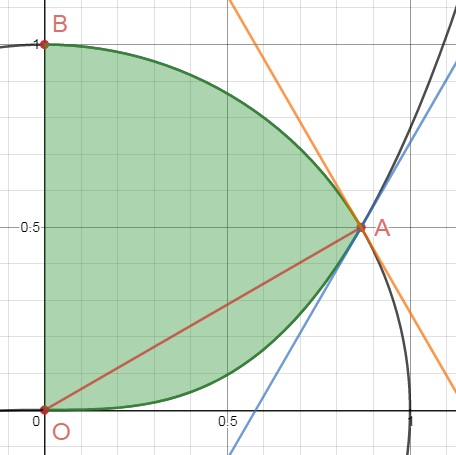
\includegraphics[width=\linewidth]{../problems/Q_193/A_193.png}
\end{wrapfigure}
面積を求める領域は図の緑で示した部分である。点B$(0,1)$をおくと、A$\left(\dfrac{\sqrt{3}}{2}, \dfrac{1}{2}\right)$であるから、$\angle\mathrm{AOB}=60^\circ$とわかる。面積を求めるにあたって、扇形OABと、線分OAと曲線C$_2$で囲まれた領域に分割して考える。線分OAは、$y=\dfrac{1}{\sqrt{3}}x$であるから、求める面積は、
\begin{align*}
 &\frac{\pi}{6}+\int^{\frac{\sqrt{3}}{2}}_0\! \left(\frac{1}{\sqrt{3}}x-\frac{4\sqrt{3}}{9}x^3 \right) \,dx \\
 =& \frac{\pi}{6}+\left[\frac{1}{2\sqrt{3}}x^2-\frac{\sqrt{3}}{9}x^4\right]^{\frac{\sqrt{3}}{2}}_0=\frac{\pi}{6}+\frac{\sqrt{3}}{16}
\end{align*}